
%% lfsr.tex
%% 2012/07/24
%% by Max Lv

\documentclass[conference]{IEEEtran}


% *** CITATION PACKAGES ***
%
\usepackage{cite}
\usepackage[dvipdfm]{hyperref}


% *** GRAPHICS RELATED PACKAGES ***
%
\usepackage{graphicx}


% *** ALIGNMENT PACKAGES ***
%
\usepackage{array}


% *** SUBFIGURE PACKAGES ***
\usepackage[tight,footnotesize]{subfigure}
%\usepackage[caption=false,font=footnotesize]{subfig}


% *** PDF, URL AND HYPERLINK PACKAGES ***
%
\usepackage{url}


% correct bad hyphenation here
\hyphenation{op-tical net-works semi-conduc-tor}


%% *** DOCUMENT BEGINS HERE ***
%
\begin{document}


\title{Local Feature Based Salient Region Detection}
\author{\IEEEauthorblockN{Chao Lv}
\IEEEauthorblockA{Parallel Processing Institute, Fudan University\\
Email: max.c.lv@gmail.com}}
\maketitle


\begin{abstract}

The abstract goes here.

\end{abstract}


\IEEEpeerreviewmaketitle


\section{Introduction}

This demo file is intended to serve as a ``starter file''
for IEEE conference papers produced under \LaTeX\ using
IEEEtran.cls version 1.7 and later.
I wish you the best of success.

\hfill mds
 
\hfill January 11, 2007

\subsection{Subsection Heading Here}

Subsection text here.


\subsubsection{Subsubsection Heading Here}

Subsubsection text here.


% An example of a floating figure using the graphicx package.
% Note that \label must occur AFTER (or within) \caption.
% For figures, \caption should occur after the \includegraphics.
% Note that IEEEtran v1.7 and later has special internal code that
% is designed to preserve the operation of \label within \caption
% even when the captionsoff option is in effect. However, because
% of issues like this, it may be the safest practice to put all your
% \label just after \caption rather than within \caption{}.
%
% Reminder: the "draftcls" or "draftclsnofoot", not "draft", class
% option should be used if it is desired that the figures are to be
% displayed while in draft mode.
%
%\begin{figure}[!t]
%\centering
%\includegraphics[width=2.5in]{myfigure}
% where an .eps filename suffix will be assumed under latex, 
% and a .pdf suffix will be assumed for pdflatex; or what has been declared
% via \DeclareGraphicsExtensions.
%\caption{Simulation Results}
%\label{fig_sim}
%\end{figure}

% Note that IEEE typically puts floats only at the top, even when this
% results in a large percentage of a column being occupied by floats.


% An example of a double column floating figure using two subfigures.
% (The subfig.sty package must be loaded for this to work.)
% The subfigure \label commands are set within each subfloat command, the
% \label for the overall figure must come after \caption.
% \hfil must be used as a separator to get equal spacing.
% The subfigure.sty package works much the same way, except \subfigure is
% used instead of \subfloat.
%
\begin{figure*}[!t]
\centerline{\subfigure[Case I]{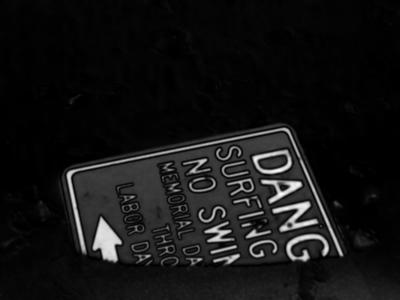
\includegraphics[width=2.5in,natwidth=400,natheight=300]{fig1.jpg}}
\hfil
\subfigure[Case II]{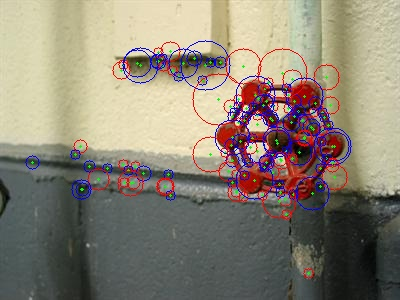
\includegraphics[width=2.5in,natwidth=400,natheight=300]{fig2.jpg}}}
\caption{Simulation results}
\end{figure*}
%
%Note that often IEEE papers with subfigures do not employ subfigure
%captions (using the optional argument to \subfloat), but instead will
%reference/describe all of them (a), (b), etc., within the main caption.


% An example of a floating table. Note that, for IEEE style tables, the 
% \caption command should come BEFORE the table. Table text will default to
% \footnotesize as IEEE normally uses this smaller font for tables.
% The \label must come after \caption as always.
%
\begin{center}
\begin{table*}[ht]
%% increase table row spacing, adjust to taste
\renewcommand{\arraystretch}{1.3}
% if using array.sty, it might be a good idea to tweak the value of
% \extrarowheight as needed to properly center the text within the cells
\caption{An Example of a Table}
\label{table_example}
%% Some packages, such as MDW tools, offer better commands for making tables
%% than the plain LaTeX2e tabular which is used here.
\centerline{\begin{tabular}{|c||c|}
\hline
AAAAAAAAAAAAAAAAAAAAAAAAAAAAAAAAAAA & BBBBBBBBBBBBBBBBBBBBBBBBBBBBBBBB\\
\hline
Three & Four\\
\hline
\end{tabular}}
\end{table*}
\end{center}


\section{Conclusion}
The conclusion goes here.


% use section* for acknowledgement
\section*{Acknowledgment}


The authors would like \cite{Gowers} to thank...


% trigger a \newpage just before the given reference
% number - used to balance the columns on the last page
% adjust value as needed - may need to be readjusted if
% the document is modified later
%\IEEEtriggeratref{8}


% references section
\bibliographystyle{IEEEtran}
\bibliography{lfsr}


% that's all folks
\end{document}


